\documentclass[../main.tex]{subfiles}
\graphicspath{{\subfix{../images/}}} % Images path

\begin{document}

\section{Image Representation}\label{sec:image-representation}

A important step in the Bag of Visual Words (BoW) pipeline is the representation
of images as fixed-length feature vectors. In this study, $4$ different
techniques have been implemented to perform this task.\\
The classic approach is to represent images as \itt{normalized histograms
of visual words (HIST)}. For each image, the previously extracted descriptors are
assigned to the closest visual word in the vocabulary, and a histogram is built
counting the occurrences of each visual word in the image. Formally, the $i$-th
bin of each histogram is computed as
\begin{equation}
	h_i = \frac{n_{id}}{n_{d}},
	\quad
	\forall i \in \{0, \ldots, K-1\},
	\forall d \in \{0, \ldots, N-1\}
\end{equation}

where 
$n_{id}$ is the number of occurrences of the $i$-th visual word in image $d$,
$n_{d}$ is the total number of visual words in the image,
and $N$ is the total number of images in the dataset.
After normalization,
the result is a fixed-length representation in which images are seen as
normalized histograms having $K$ bins, corresponding to visual words
frequencies.\\
In order to account for the relevance of the visual words, another idea is to
use the \itt{term frequency-inverse document frequency (TF-IDF)} weighting
scheme. In this case, given the number of images $N_i$ containing the $i$-th
visual word, the histogram bins are
\begin{equation}
	h_i = \frac{n_{id}}{n_{d}} \cdot \log\left(\frac{N}{N_i}\right),
	\quad 
	\forall i \in \{0, \ldots, K-1\}, 
	\forall d \in \{0, \ldots, N-1\}
\end{equation}

A third approach is to use the \itt{soft assignment} techniques proposed by
\itt{Van Gemert et al.}~\cite{gemert}, which argue that the hard assignment of
visual words to descriptors gives rise to two types of ambiguity: \itt{codeword
uncertainty} when a descriptor is similarly close to two or more visual words,
and \itt{codeword plausibility} when a descriptor is relatively far from all
visual words.
To address this issue, the authors propose the usage of a Gaussian kernel
$K_{\sigma}(x)$  density estimator\footnote{See Appendix
\ref{app:kernel-density-estimation}.} based on the Euclidean distance $D(w_i,
x_j)$ between each $i$-th visual word $w_i$ and $j$-th descriptor $x_j$ to
approximate the probability density function of visual words in the images.
Hence, by replacing the histogram estimator with
the kernel density estimator the result is the \itt{kernel codebook (KCB)}
representation, in which each descriptor can contribute to multiple bins
according to the equation
\begin{equation}\label{eq:kcb}
	h_i = \frac{1}{n_{ri}} \sum_{j=0}^{n_{ri}} K_{\sigma}(D(w_i, x_j)),
	\quad
	\forall i \in \{0, \ldots, K-1\},
	\forall d \in \{0, \ldots, N-1\}
\end{equation}

A visual comparison between the representations obtain with hard
assignment and soft assignment methods for a sample image is shown in
Figure~\ref{fig:hist-kcb-example}.
According to the authors, this soft assignment strategy models the two types of
ambiguity at the same time, but it's also possible to consider them separately
by adopting either the \itt{codeword uncertainty (UNC)} representation
\begin{equation}\label{eq:unc}
	h_i = \frac{1}{n_{ri}}
	\sum_{j=0}^{n_{ri}} \frac{K_{\sigma}(D(w_i, x_j))}{\sum_{l=0}^{K-1}
	K_{\sigma}(D(w_l, x_j))},
\end{equation}

or the \itt{codeword plausibility (PLA)} representation
\begin{equation}\label{eq:pla}
	h_i = \frac{1}{n_{ri}}
	\sum_{j=0}^{n_{ri}}
	\begin{cases}
		K_{\sigma}(D(w_i, x_j)), & \text{if } w_i = \underset{l \in \{0, \ldots, K-1\}}{\text{argmin}} D(w_l, x_j)\\
		0, & \text{otherwise}
	\end{cases}
\end{equation}

Notice that in equations~\ref{eq:kcb}, \ref{eq:unc}, and \ref{eq:pla} the sums are not performed for all the
$n_{d}$ descriptors in the image, but only over the $n_{ri}$ descriptors in the
region around the $i$-th visual word. 
In the original paper, in fact, the authors employed \itt{radius based} clustering to construct the visual vocabulary. 
Since in this study \itt{k-means} has been used, an approximation of each
cluster radius has been obtained as the maximal distance\footnote{In Euclidean
norm} between the cluster centroid and the descriptors assigned to it. The
region around each visual word is hence defined as the set of descriptors whose
distance from the centroid is less than the corresponding radius. Such
definition possibly implies overlapping regions, meaning that a descriptor can
belong to more than one region, and empirically led to better
results than including all the descriptors in the image in the computation.

\begin{figure}[htb]
  \centering
  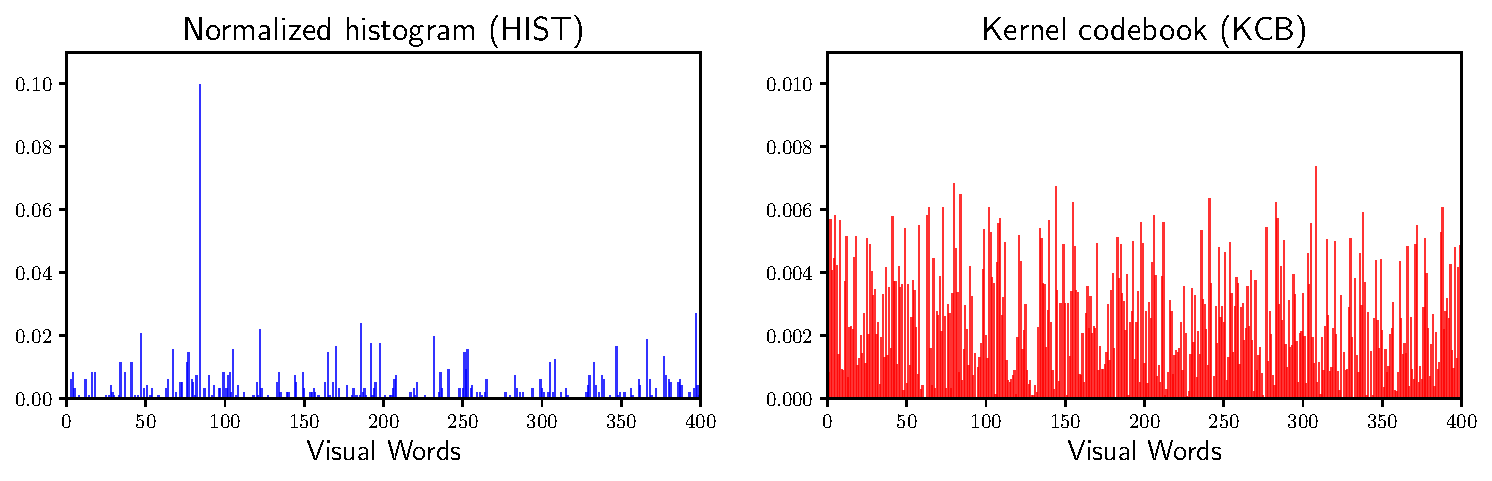
\includegraphics[width=\textwidth]{representations_comparison.pdf}
  \caption{Comparison between normalized histogram (\itt{blue}) and kernel
  codebook (\itt{red}) representations for image $1200$ in train set.}\label{fig:hist-kcb-example}
\end{figure}


\pagebreak
The last approach used to fulfill the image representation task is the
use of \itt{spatial pyramid matching (SPM)} method proposed by \itt{Lazebnik et
al.}~\cite{lazebnik}. 
The idea is to repeatedly subdivide each image into
subsequently finer grids at different resolution levels $\ell \in
\{0,\dots,L-1\}$, and to compute the histograms $H_{\ell}(g)$ of visual words
for each $g$-th grid at level $\ell$. Precisely, at level $\ell$ each
image is divided into $2^{\ell}$ cells along each dimension, and the count of
visual words is computed for each cell.
All the histograms are then weighted according to the weighting
scheme in equation~\ref{eq:spm-weights},
that favors features counts computed at higher levels
of the pyramid. 
% In particular, if $L$ is
% the number of levels in the pyramid, the weights multiplying histograms
% at level $\ell$ are computed as
\begin{equation}\label{eq:spm-weights}
	\omega_0 = \frac{1}{2^{L}},
	\quad
	\omega_{\ell} = \frac{1}{2^{L-\ell+1}},
	\quad
	\forall \ell \in \{0, \ldots, L-1\}
\end{equation}

The resulting weighted histograms are then stacked together to form, for each
image, a single \itt{extended multi-level descriptor}
% that can be used as input to the SVM classifiers presented in Section~\ref{sec:classification}.
% Such descriptor, 
% that not only contains the information about the visual words, but also
% encodes positional information at different scales which was missing in the
% standard BoW approach.\\
that encodes both visual words and positional information at different
scales and can be used as input to SVM classifiers.
The idea of using SVM classifiers specifically for this representation comes
from the possibility of adopting the \itt{spatial pyramid kernel} in order to
compute the similarity between these extended descriptors by correctly measuring
the information at different levels of the pyramid. Formally, given two images
$X$ and $Y$ represented by their extended descriptors of elements
$H^{X}_{\ell, i}(g)$ and $H^{Y}_{\ell, i}(g)$,
% \begin{equation*}
%   \begin{aligned}
% 	H^{X} &= \{H_{\ell, i}^{X}(g) \mid  \forall \ell \in \{0,\dots,L-1\}, \forall i \in \{0,\dots,K-1\}, \forall g \in \{0,\dots,2^{2 \ell}-1\}\} \\
% 	H^{Y} &= \{H_{\ell, i}^{Y}(g) \mid  \forall \ell \in \{0,\dots,L-1\}, \forall i \in \{0,\dots,K-1\}, \forall g \in \{0,\dots,2^{2 \ell}-1\}\}
%   \end{aligned}
% \end{equation*}
the \itt{pyramid match kernel} between the two is 
\begin{equation}
  K^{L}(X,Y) = 
  \sum_{\ell=0}^{L-1}
  \sum_{i=0}^{K-1}
  \sum_{g=0}^{2^{2 \ell}-1}
  \min\left(H_{\ell, i}^{X}(g), H_{\ell, i}^{Y}(g)\right)
\end{equation}

which can be efficiently computed as a simple histogram intersection kernel.\\
Finally, it's important to notice that for this last representation the features
are extracted from images only by using the grid approach. This has been done
both to follow the same approach of the original paper and also to avoid the
possibility of having empty cells which might happen for those containing
uniform regions of the image\footnote{E.g.\ cells positioned in the top region
	of the left side image or in the bottom left corner of the right side
image in Figure~\ref{fig:keypoints-example}.}.

\end{document}

